\documentclass[compress,aspectratio=1610, xcolor=table]{beamer}
\usepackage{xcolor}
\renewcommand<>\cellcolor[1]{\only#2{\beameroriginal\cellcolor{#1}}}
%new header 
% This example is meant to be compiled with lualatex or xelatex
% The theme itself also supports pdflatex
\PassOptionsToPackage{unicode}{hyperref}
%\documentclass[aspectratio=1610, 9pt]{beamer}

% Load packages you need here
\usepackage{polyglossia}
\usefonttheme{professionalfonts}
%\setmainlanguage{english}

\usepackage{csquotes}
    
\usepackage{appendixnumberbeamer}

\usepackage{amsmath}
\usepackage{amssymb}
\usepackage{mathtools}

\usepackage{hyperref}
\usepackage{bookmark}

% Paket float verbessern
\usepackage{scrhack}

% Warnung, falls nochmal kompiliert werden muss

% unverzichtbare Mathe-Befehle
\usepackage{amsmath}
% viele Mathe-Symbole
\usepackage{amssymb}
% Erweiterungen für amsmath
\usepackage{mathtools}

% Fonteinstellungen
\usepackage{fontspec}
% Latin Modern Fonts werden automatisch geladen
% Alternativ:
%\setromanfont{Libertinus Serif}
%\setsansfont{Libertinus Sans}
%\setmonofont{Libertinus Mono}
% sollte man das Seiten-Layout neu berechnen lassen

% deutsche Spracheinstellungen
%\usepackage{polyglossia}
\setmainlanguage{english}

\usepackage[
  math-style=ISO,    % ┐
  bold-style=ISO,    % │
  sans-style=italic, % │ ISO-Standard folgen
  nabla=upright,     % │
  partial=upright,   % ┘
  warnings-off={           % ┐
    mathtools-colon,       % │ unnötige Warnungen ausschalten
    mathtools-overbracket, % │
  },                       % ┘
]{unicode-math}

% Zahlen und Einheiten
\usepackage[
  locale=UK,                   % deutsche Einstellungen
  separate-uncertainty=true,   % immer Fehler mit \pm
  per-mode=symbol-or-fraction, % / in inline math, fraction in display math
]{siunitx}

% schöne Brüche im Text
\usepackage{xfrac}

% Standardplatzierung für Floats einstellen
\usepackage{float}
\floatplacement{figure}{H}
\floatplacement{table}{H}

% Floats innerhalb einer Section halten
\usepackage[
  section, % Floats innerhalb der Section halten
  below,   % unterhalb der Section aber auf der selben Seite ist ok
]{placeins}

%dassselbe für Subsections 
\makeatletter
\AtBeginDocument{%
  \expandafter\renewcommand\expandafter\subsection\expandafter{%
    \expandafter\@fb@secFB\subsection
  }%
}
\makeatother

% Seite drehen für breite Tabellen: landscape Umgebung
% \usepackage{pdflscape}

% Captions schöner machen.
% \usepackage[
%   labelfont=bf,        % Tabelle x: Abbildung y: ist jetzt fett
%   font=small,          % Schrift etwas kleiner als Dokument
%   width=0.7\textwidth, % maximale Breite einer Caption schmaler
% ]{caption}

% Die Einstellung ist in Konflikt mit der in der Tu Vorlage.
% Dadurch respektieren die Captions die Breite einer
% umgebenden minipage nicht mehr


% subfigure, subtable, subref
\usepackage{subcaption}

% Grafiken können eingebunden werden
\usepackage{graphicx}
% größere Variation von Dateinamen möglich
%\usepackage{grffile}

% schöne Tabellen
\usepackage{booktabs}

% Verbesserungen am Schriftbild
\usepackage{microtype}

% Literaturverzeichnis
% \usepackage[
%   sorting=none,%authortitle,
%   autolang=hyphen,
%   style=authortitle,
%   backend=biber,
% ]{biblatex}

\usepackage[
  % style=numeric,
  % style=authoryear-ibid,
  % style=verbose,
  doi=false,
  style=phys,
  % sorting=none,
  backend=biber,
  autolang=hyphen,
  articletitle=false,
  chaptertitle=false,
  biblabel=brackets,
  eprint=false,
  pageranges=false,
  doi=false,
  % useauthor=false,
]{biblatex}
% Quellendatenbank
\addbibresource{lit.bib}
% \AtEveryBibitem{\clearname{author}}
% \AtEveryCitekey{\clearname{author}}
% \renewbibmacro*{byauthor}{}
% \renewbibmacro*{author}{}
\DeclareFieldFormat{author}{}


% Hyperlinks im Dokument

% Trennung von Wörtern mit Strichen
\usepackage[shortcuts]{extdash}

%selbst hinzugefügt
\usepackage{physics}

% load the theme after all packages

\usetheme{tu}

% Put settings here, like
\unimathsetup{
  math-style=ISO,
  bold-style=ISO,
  nabla=upright,
  partial=upright,
  mathrm=sym,
}
\renewcommand{\thefigure}{\hspace{-.333333em}}


% traditionelle Fonts für Mathematik
\setmathfont{Latin Modern Math}
% Alternativ:
%\setmathfont{Libertinus Math}
\setmathfont{XITS Math}[range={scr, bfscr}]
\setmathfont{XITS Math}[range={cal, bfcal}, StylisticSet=1]

\newcommand{\jpsi}{\ensuremath{J \! / \! \psi}}
\newcommand{\bs}{\ensuremath{B^0_s}}
\newcommand{\bd}{\ensuremath{B^0}}
\newcommand{\pp}{\ensuremath{p\bar{p}}}
\newcommand{\jpsipp}{\ensuremath{B^0_{(s)} \rightarrow \jpsi p\bar{p}}}
\newcommand{\ppmm}{\ensuremath{B^0_{(s)} \rightarrow p\bar{p}\mu^+\mu^-}}
\newcommand{\br}[1]{\ensuremath{\mathcal{B}(#1)}}
\newcommand{\ppmumu}{\ensuremath{p\bar{p}\mu^+\mu^-}}
\newcommand{\bsppmm}{\ensuremath{\bs\rightarrow\ppmumu}}
\newcommand{\bdppmm}{\ensuremath{\bd\rightarrow\ppmumu}}

\newcommand{\jpsippnew}{\ensuremath{}{\jpsi p\bar{p}}}
\newcommand{\bsjpsipp}{\ensuremath{\bs\rightarrow\jpsippnew}}
\newcommand{\bdjpsipp}{\ensuremath{\bd\rightarrow\jpsippnew}}
\newcommand{\jpsiphi}{\ensuremath{\bs\rightarrow\jpsi\phi}}
\renewcommand\thefootnote{[\arabic{footnote}]}


\DeclareSourcemap{
 \maps[datatype=bibtex,overwrite=true]{
  \map{
    \step[fieldsource=Collaboration, final=true]
    \step[fieldset=usera, origfieldval, final=true]
  }
 }
}

% \renewbibmacro*{author}{%
%   \iffieldundef{usera}{
%     \printnames{author}
%   }{
%     \printfield{usera}
%   }
% }
% \setbeamercolor{bibliography item}{parent=palette primary}
% \setbeamercolor{bibliography}{parent=palette primary}
% \setbeamercolor*{bibliography entry title}{parent=palette primary}
\setbeamercolor{bibliography entry author}{fg=darkgray, bg=white}
\setbeamercolor{bibliography entry title}{fg=darkgray, bg=white}
\setbeamercolor{bibliography entry note}{fg=darkgray, bg=white}

\DeclareSIUnit\gev{\giga\electronvolt}
\DeclareSIUnit\clight{\text{\ensuremath{c}}}
\DeclareSIUnit\eVperc{\eV\per\clight}
\DeclareSIUnit\mass{\mega\eVperc\squared}

\usepackage[beamer,customcolors]{hf-tikz}

\tikzset{hl/.style={
    set fill color=red!80!black!40,
    set border color=red!80!black,
  },
}

\makeatletter
% % Default:
% \def\@makefnmark{\hbox{\@textsuperscript{\normalfont\@thefnmark}}}
\renewcommand{\@makefnmark}{\makebox{\normalfont \@thefnmark}}
\makeatother
\title[Bird Species Classification]{Bird Species Classification Using Audio Signal Processing and Convolutional Neural Networks}
\subtitle{Machine Learning Seminar (not Lecture)}
\date[6 June 2024]{6th of June, 2024}
\author[L.~Bertsch and T.~Troska]{Lukas Bertsch and Tom Troska}
\institute[TU Dortmund]{TU Dortmund - Faculty of Physics}
\titlegraphic{
  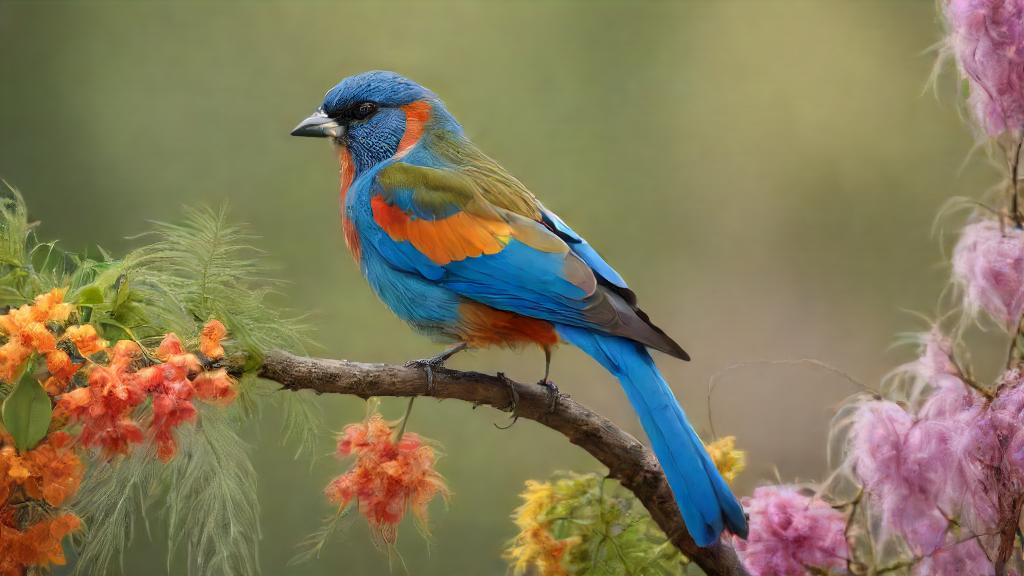
\includegraphics[width=0.65\textwidth]{images/bird.jpg}
  }
\sisetup
  {
  list-exponents = combine-bracket ,
  product-exponents = combine-bracket ,
  range-exponents = combine-bracket
  }
\usepackage{caption}
\captionsetup[figure]{labelformat=empty}
\usepackage{tikz}
\usepackage[compat=1.1.0]{tikz-feynman} 
\AtBeginDocument{\RenewCommandCopy\qty\SI}

%\input{feynmans.tex}

\begin{document}

\maketitle

\begin{frame}{Problem}
  %\textcolor{tugreen}{\Large Problem:}
  \begin{itemize}
    \item How effectively can we classify bird species by analysing sound files using a convolutional neural network (CNN)?
  \end{itemize}
  \vspace{2mm}
  \textcolor{tugreen}{\Large Motivation:}
  \vspace{1mm}
  \begin{itemize}
    \item Classifying and observing different species of birds is of great interest for wildlife research
    \item But often you don't see the birds themselves and only hear their calls
    \item Differentiating bird species from sound recordings requires expert knowledge and is very time consuming
    \begin{columns}
      \column{.45\textwidth}
      \vspace*{-3mm}
      \begin{itemize}
        \item A CNN could be used to automatically identify different species by patterns in spectrograms of audio recordings
      \end{itemize}

      \column{.55\textwidth}
      \vspace{-2mm}
      \begin{figure}
        \centering
        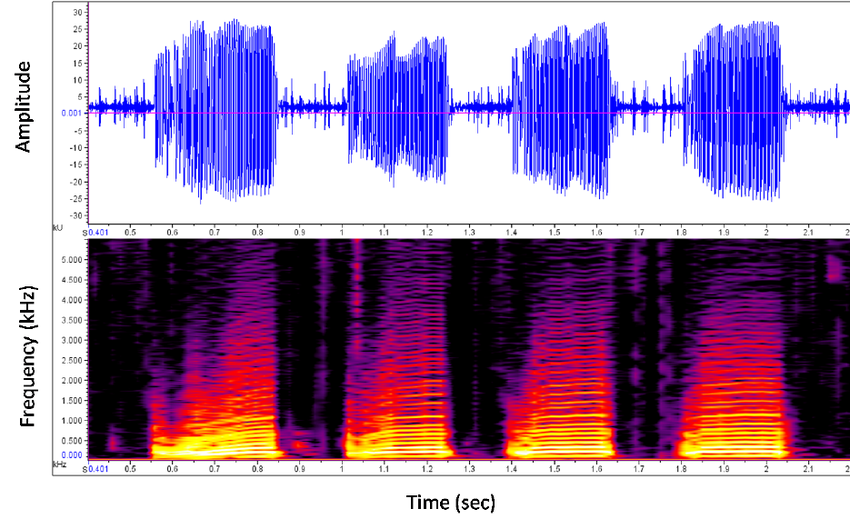
\includegraphics[width = .6\textwidth]{content/graphics/spectrogram.png}
        \caption*{\scriptsize \fullcite{Kat2009}}
      \end{figure}
    \end{columns}
  \end{itemize}
\end{frame}

\begin{frame}{Dataset}
  \only<1>{
  \vspace*{-16mm}
  \begin{itemize}
    \item Source: \href{https://www.kaggle.com/datasets/monogenea/birdsongs-from-europe}{\textcolor{blue}{www.kaggle.com/datasets/monogenea/birdsongs-from-europe}}
    \item Dataset contains sound recordings of 50 european bird species
    \begin{itemize}
      \item For each species there are $\num{43}$ .mp3 files of different length
      \item The recordings contain background noises etc. 
    \end{itemize}
    \item Additionally, a .csv file with metadata for all recordings is provided
    \begin{itemize}
      \item Species, location, recordist, date ...
    \end{itemize}
  \end{itemize}
  }
  \begin{figure}
    \centering 
    \includegraphics<2>[width=\textwidth]{content/graphics/dataframe.png}
  \end{figure}
  \only<3>{
    \vspace*{-16mm}
    \begin{itemize}
      \item Source: \href{https://www.kaggle.com/datasets/monogenea/birdsongs-from-europe}{\textcolor{blue}{www.kaggle.com/datasets/monogenea/birdsongs-from-europe}}
      \item Dataset contains sound recordings of 50 european bird species
      \begin{itemize}
        \item For each species there are $\num{43}$ .mp3 files of different length
        \item The recordings contain background noises etc. 
      \end{itemize}
      \item Additionally, a .csv file with metadata for all recordings is provided
      \begin{itemize}
        \item Species, location, recordist, date ...
      \end{itemize}
      \item Original data from \href{https://xeno-canto.org/}{\textcolor{blue}{xeno-canto.org/}}
      \begin{itemize}
        \item A website for sharing and classifying wildlife sound recordings
      \end{itemize}
      \item Each audio file is licensed individually by its author
      \begin{itemize}
        \item The individual licenses are listed in the .csv 
        \item Different \textit{Creative Commons} licenses (free for non-commercial use)
      \end{itemize}
    \end{itemize}
  }
\end{frame}

\begin{frame}{Comparison with alternative method}
  \begin{itemize}
    \item Using a CNN is the most obvious and most promising approach for such a problem 
    \item An alternative method could e.g. make use of a \textit{KNN} classifier
  \end{itemize}
  \vspace{2mm}
  \textcolor{tugreen}{\large Strategy:}
  \begin{enumerate}
    \item Extract meaningful features from the audio files 
    \begin{itemize}
      \item Zero crossing rate, RMS energy (loudness), energy
      \item Spectral analysis using \textit{FFT} or \textit{Lomb-Scargle}
      \item Most prominent frequencies, spectral centroid/flux/spread etc.
    \end{itemize}
    \item Train k-nearest neighbours algorithm 
    \item Compare performance
  \end{enumerate}
  \vspace{2mm}
  \textcolor{tugreen}{\large Performance measure:}
  \begin{itemize}
    \item Accuracy / F1-score
  \end{itemize}
\end{frame}


\end{document}

